\documentclass{beamer}
\usepackage[english, russian]{babel}
\usepackage[T2A]{fontenc}
\usepackage[utf8]{inputenc}
\usepackage{indentfirst}
\usepackage{amsmath, amsfonts, amssymb, amsthm, mathtools}
\usepackage[export]{adjustbox}
\usepackage{graphicx} 
\graphicspath{ {./images/} }

\usepackage{subcaption}
\usepackage{verbatim}

\usepackage{minted}{\setlength{\parskip}{0pt}}

\usepackage{hyperref}

\hypersetup{
    colorlinks=true,
    linkcolor=blue,
    filecolor=magenta,      
    urlcolor=black,
    pdftitle={Overleaf Example},
    pdfpagemode=FullScreen,
    }


\title{Отчет по лабораторной работе № 14. \\ Настройка файловых служб Samba}
\author{Данила Стариков \\ НПИбд-02-22}
\date{2024}

\begin{document}

\maketitle
\newpage
\tableofcontents

\newpage
\section{Цель работы}
Приобретение навыков настройки доступа групп пользователей к общим ресурсам по протоколу SMB.
\newpage

\section{Выполнение работы}
\subsection{Настройка сервера Samba}
\begin{enumerate}
\item На сервере установили необходимые пакеты:
    \begin{minted}{bash}
dnf -y install samba samba-client cifs-utils
    \end{minted}
\item Создали группу {\tt sambagroup} для пользователей, которые будут работать с {\tt Samba}-сервером, и присвоили ей GID 1011 (Рис. \ref{img:01}):
    \begin{minted}{bash}
groupadd -g 1010 sambagroup
    \end{minted}
\item Добавили пользователя {\tt dastarikov} к группе {\tt sambagroup} (Рис. \ref{img:01}):
    \begin{minted}{bash}
usermod -aG sambagroup dastarikov
    \end{minted}

\begin{center}
    \centering
    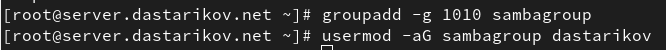
\includegraphics[width=0.8\textwidth]{../images/image01.png}
    \captionof{figure}{Создание группы sambagroup и добавления в нее пользователя dastarikov.}
    \label{img:01}
\end{center}

\item Создали общий каталог в файловой системе {\tt Linux}, в который предполагается монтировать разделяемые ресурсы:
    \begin{minted}{bash}
mkdir -p /srv/sambashare
    \end{minted}
\item В файле конфигурации {\tt /etc/samba/smb.conf} (Рис. \ref{img:27}):
    \begin{enumerate}
        \item изменили параметр рабочей группы:
    \begin{minted}{bash}
[global]
workgroup = DASTARIKOV-NET
    \end{minted}
    и добавили сразу после строки {\tt workgroup} поля для работы через SMB1 протокол:
    \begin{minted}{bash}
server min protocol = NT1
client min protocol = NT1
    \end{minted}
\item в конце файла добавили раздел с описанием общего доступа к разделяемому ресурсу {\tt /srv/sambashare}:
    \begin{minted}{bash}
[sambashare]
comment = My Samba Share
path = /srv/sambashare
write list = @sambagroup
    \end{minted}

\begin{center}
    \centering
    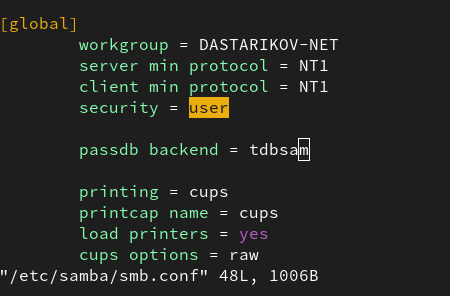
\includegraphics[width=0.8\textwidth]{../images/image27.png}
    \captionof{figure}{Изменение конфигурации samba на сервере.}
    \label{img:27}
\end{center}

    \end{enumerate}
\item Убедились, что не сделали синтаксических ошибок в файле {\tt smb.conf}, используя команду (Рис. \ref{img:02}):
    \begin{minted}{bash}
testparm
    \end{minted}

\begin{center}
    \centering
    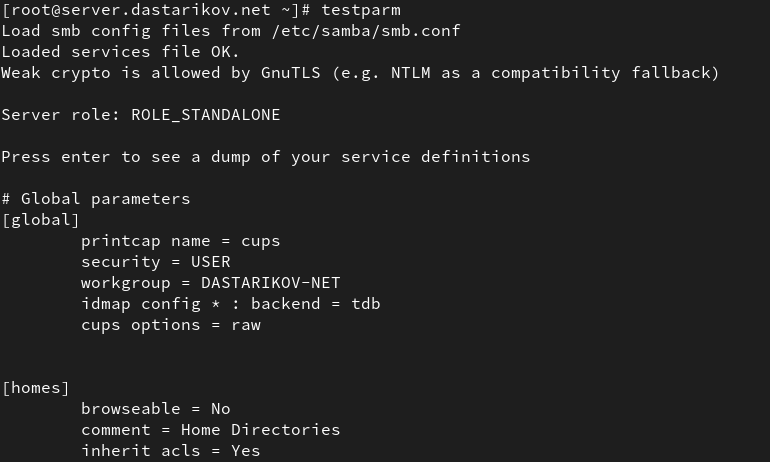
\includegraphics[width=0.8\textwidth]{../images/image02.png}
    \captionof{figure}{Проверка правильности синтаксиса файла samba.conf.}
    \label{img:02}
\end{center}

\item Запустили демон {\tt Samba} и посмотрите его статус (Рис. \ref{img:03}):
    \begin{minted}{bash}
systemctl start smb
systemctl enable smb
systemctl status smb
    \end{minted}

\begin{center}
    \centering
    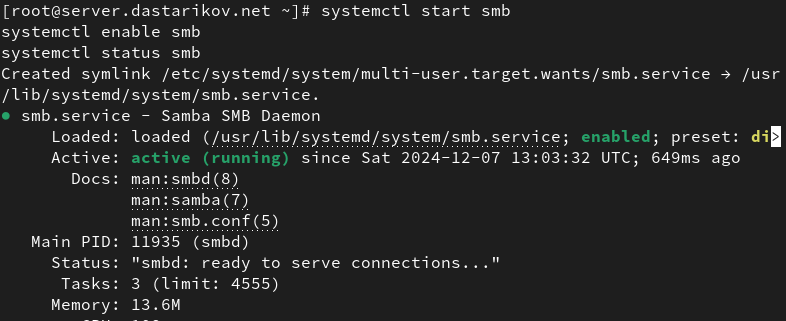
\includegraphics[width=0.8\textwidth]{../images/image03.png}
    \captionof{figure}{Включение демона Samba.}
    \label{img:03}
\end{center}

\item Для проверки наличия общего доступа подключились к серверу с помощью {\tt smbclient} (Рис. \ref{img:16}):
    \begin{minted}{bash}
smbclient -L //server
    \end{minted}
(при запросе пароля нажмите {\tt Enter} для работы под анонимным пользователем).

\begin{center}
    \centering
    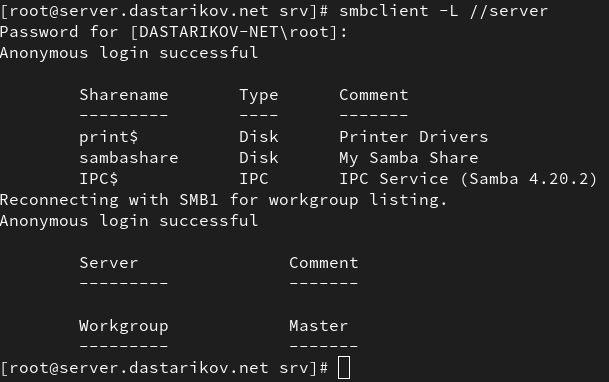
\includegraphics[width=0.8\textwidth]{../images/image16.png}
    \captionof{figure}{Проверка наличия общего доступа к серверу.}
    \label{img:16}
\end{center}

\item Посмотрели файл конфигурации межсетевого экрана для {\tt Samba} (Рис. \ref{img:04}):
    \begin{minted}{bash}
less /usr/lib/firewalld/services/samba.xml
    \end{minted}

\begin{center}
    \centering
    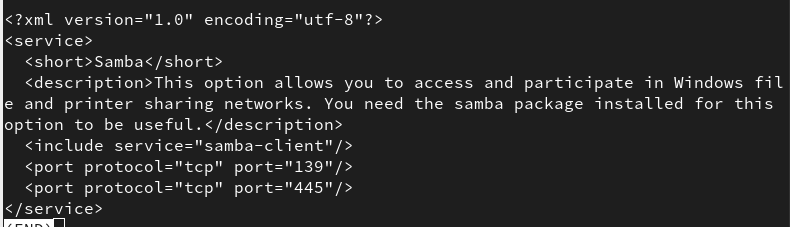
\includegraphics[width=0.8\textwidth]{../images/image04.png}
    \captionof{figure}{Просмотр конфигурации межсетевого экрана Samba.}
    \label{img:04}
\end{center}

\item Настроили межсетевой экран (Рис. \ref{img:05}):
    \begin{minted}{bash}
firewall-cmd --add-service=samba
firewall-cmd --add-service=samba --permanent
firewall-cmd --reload
    \end{minted}

\begin{center}
    \centering
    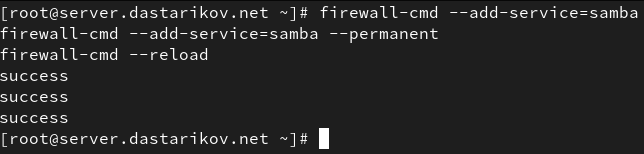
\includegraphics[width=0.8\textwidth]{../images/image05.png}
    \captionof{figure}{Настройка межсетевого экрана.}
    \label{img:05}
\end{center}

\item Настроили права доступа для каталога с разделяемым ресурсом (Рис. \ref{img:06}):
    \begin{minted}{bash}
chgrp sambagroup /srv/sambashare
chmod g=rwx /srv/sambashare
    \end{minted}
\item Посмотрели контекст безопасности {\tt SELinux} (Рис. \ref{img:06}):
    \begin{minted}{bash}
cd /srv
ls -Z
    \end{minted}

\begin{center}
    \centering
    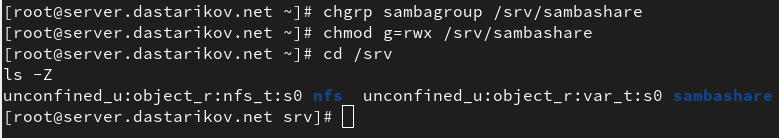
\includegraphics[width=0.8\textwidth]{../images/image06.png}
    \captionof{figure}{Настройка прав доступа для каталога с разделяемым ресурсом sambashare.}
    \label{img:06}
\end{center}

\item Настроили контекст безопасности {\tt SELinux} для каталога с разделяемым ресурсом (Рис. \ref{img:08}):
    \begin{minted}{bash}
semanage fcontext -a -t samba_share_t "/srv/sambashare(/.*)?"
restorecon -vR /srv/sambashare
    \end{minted}
\item Проверили, что контекст безопасности изменился (Рис. \ref{img:08}):
    \begin{minted}{bash}
cd /srv
ls -Z
    \end{minted}

\begin{center}
    \centering
    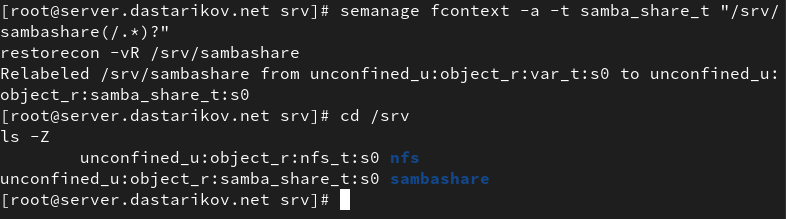
\includegraphics[width=0.8\textwidth]{../images/image08.png}
    \captionof{figure}{Настройка SELinux для каталога с разделяемым ресурсом smbshare.}
    \label{img:08}
\end{center}

\item Разрешили экспортировать разделяемые ресурсы для чтения и записи (Рис. \ref{img:09}):
    \begin{minted}{bash}
setsebool samba_export_all_rw 1
setsebool samba_export_all_rw 1 -P
    \end{minted}

\begin{center}
    \centering
    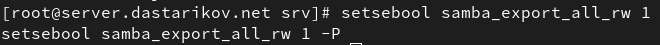
\includegraphics[width=0.8\textwidth]{../images/image09.png}
    \captionof{figure}{Настройка разрешений через флаги SELinux.}
    \label{img:09}
\end{center}

\item Посмотрели {\tt UID} вашего пользователя и в какие группы он включён (Рис. \ref{img:10}):
    \begin{minted}{bash}
id
    \end{minted}

\begin{center}
    \centering
    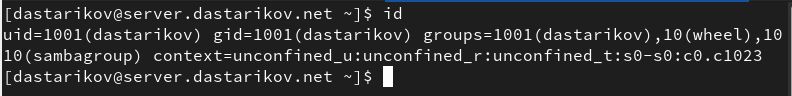
\includegraphics[width=0.8\textwidth]{../images/image10.png}
    \captionof{figure}{Просмотр групп пользователя dastarikov.}
    \label{img:10}
\end{center}

\item Под пользователем dastarikov создали файл на разделяемом ресурсе (Рис. \ref{img:11}):
    \begin{minted}{bash}
cd /srv/sambashare
touch dastarikov@server.txt
    \end{minted}

\begin{center}
    \centering
    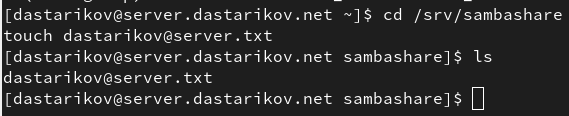
\includegraphics[width=0.8\textwidth]{../images/image11.png}
    \captionof{figure}{Создание файла на разделяемой ресурсе.}
    \label{img:11}
\end{center}

\item Добавили пользователя dastarikov в базу пользователей {\tt Samba} (Рис. \ref{img:12}):
    \begin{minted}{bash}
smbpasswd -L -a dastarikov
    \end{minted}

\begin{center}
    \centering
    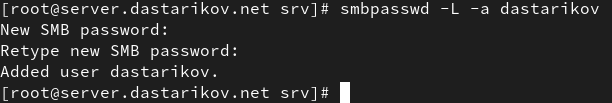
\includegraphics[width=0.8\textwidth]{../images/image12.png}
    \captionof{figure}{Добавление dastarikov в базу пользователей Samba.}
    \label{img:12}
\end{center}

\end{enumerate}

\subsection{Монтирование файловой системы Samba на клиенте}
\begin{enumerate}
\item На клиенте установили необходимые пакеты:
    \begin{minted}{bash}
dnf -y install samba-client cifs-utils
    \end{minted}
\item На клиенте посмотрели файл конфигурации межсетевого экрана для клиента {\tt Samba} (Рис. \ref{img:13}):
\begin{minted}{bash}
less /usr/lib/firewalld/services/samba-client.xml
\end{minted}

\begin{center}
    \centering
    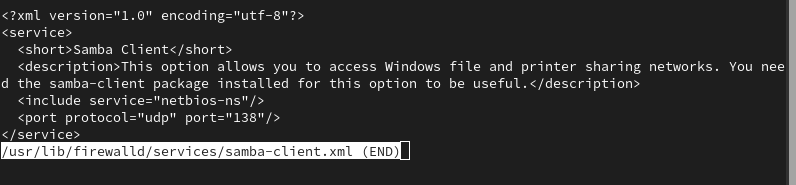
\includegraphics[width=0.8\textwidth]{../images/image13.png}
    \captionof{figure}{Просмотр конфигурации межсетевого экрана для клиента Samba.}
    \label{img:13}
\end{center}

\item На клиенте настроили межсетевой экран (Рис. \ref{img:14}):
    \begin{minted}{bash}
firewall-cmd --add-service=samba-client
firewall-cmd --add-service=samba-client --permanent
firewall-cmd --reload
    \end{minted}

\begin{center}
    \centering
    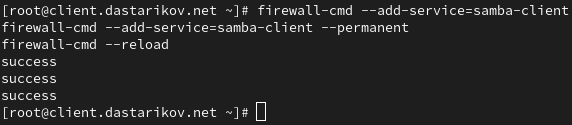
\includegraphics[width=0.8\textwidth]{../images/image14.png}
    \captionof{figure}{Настройка межсетевого экрана клиента.}
    \label{img:14}
\end{center}

\item На клиенте создали группу {\tt sambagroup} и добавили в неё пользователя {\tt dastarikov} (Рис. \ref{img:15}):
    \begin{minted}{bash}
groupadd -g 1010 sambagroup
usermod -aG sambagroup dastarikov
    \end{minted}

\begin{center}
    \centering
    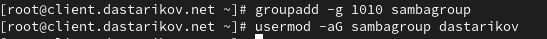
\includegraphics[width=0.8\textwidth]{../images/image15.png}
    \captionof{figure}{Создание аналогичной группы на клиенте и добавления в нее dastarikov.}
    \label{img:15}
\end{center}

\item На клиенте в файле конфигурации {\tt /etc/samba/smb.conf} изменили параметр рабочей группы (Рис. \ref{img:17}):
    \begin{minted}{bash}
[global]
workgroup = DASTARIKOV-NET
    \end{minted}
    и добавили сразу после строки {\tt workgroup} поля для работы через SMB1 протокол:
    \begin{minted}{bash}
client min protocol = NT1
    \end{minted}

\begin{center}
    \centering
    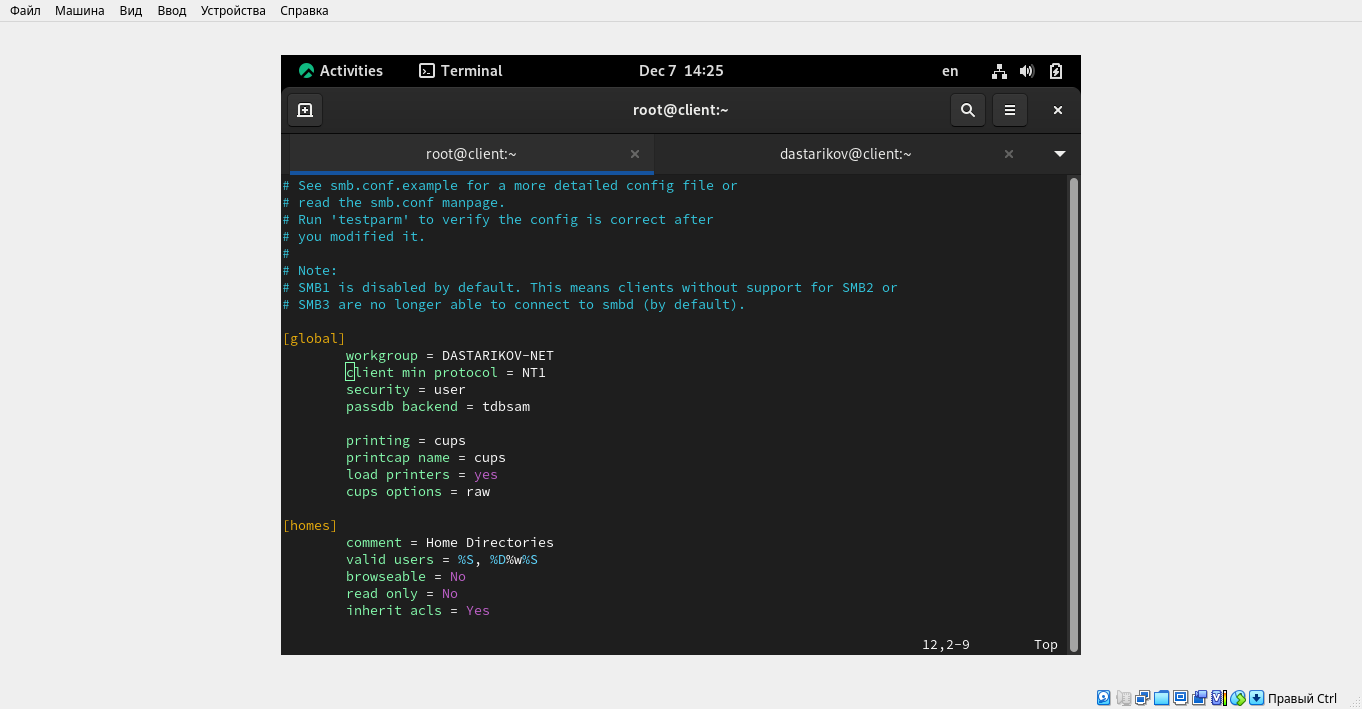
\includegraphics[width=0.8\textwidth]{../images/image17.png}
    \captionof{figure}{Изменение конфигурации samba на клиенте.}
    \label{img:17}
\end{center}

\item Для проверки наличия общего доступа подключились с клиента к серверу с помощью {\tt smbclient} под пользователем root (Рис. \ref{img:18}):
    \begin{minted}{bash}
smbclient -L //server
    \end{minted}

\begin{center}
    \centering
    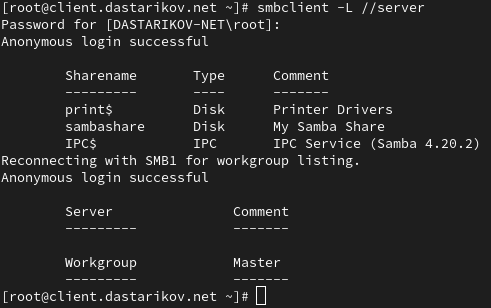
\includegraphics[width=0.8\textwidth]{../images/image18.png}
    \captionof{figure}{Подключение к серверу под пользователем root.}
    \label{img:18}
\end{center}

\item Подключились с клиента к серверу с помощью {\tt smbclient} под учётной записью своего пользователя под пользователем dastarikov (Рис. \ref{img:19}):
    \begin{minted}{bash}
smbclient -L //server -U dastarikov
    \end{minted}

\begin{center}
    \centering
    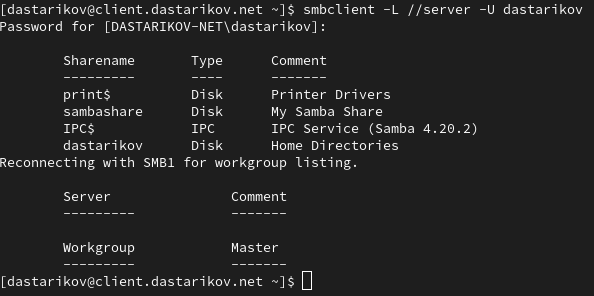
\includegraphics[width=0.8\textwidth]{../images/image19.png}
    \captionof{figure}{Подключение к серверу под пользователем dastarikov.}
    \label{img:19}
\end{center}

\item На клиенте создали точку монтирования (Рис. \ref{img:20}):
    \begin{minted}{bash}
mkdir /mnt/samba
    \end{minted}
\item На клиенте получили доступ к общему ресурсу с помощью {\tt mount} (Рис. \ref{img:20}):
    \begin{minted}{bash}
mount -o username=dastarikov,user,rw,uid=dastarikov,gid=sambagroup //server/sambashare /mnt/samba
    \end{minted}
При появлении запроса пароля ввели пароль SMB-пользователя.

\begin{center}
    \centering
    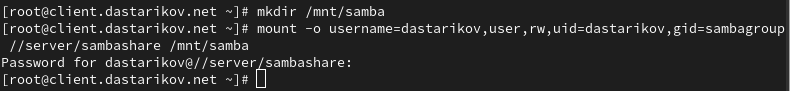
\includegraphics[width=0.8\textwidth]{../images/image20.png}
    \captionof{figure}{Монтирование разделяемого ресурса на клиенте.}
    \label{img:20}
\end{center}

\item Убедились, что {\tt dastarikov} может записывать файлы на разделяемом ресурсе (Рис. \ref{img:21}):
    \begin{minted}{bash}
cd /mnt/samba
touch dastarikov@client.txt
    \end{minted}

\begin{center}
    \centering
    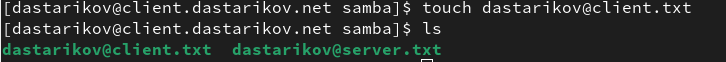
\includegraphics[width=0.8\textwidth]{../images/image21.png}
    \captionof{figure}{Проверка возможности создавать файлы на разделяемом ресурсе.}
    \label{img:21}
\end{center}

\item Отмонтировали каталог {\tt /mnt/samba} (Рис. \ref{img:22}):
    \begin{minted}{bash}
umount /mnt/samba
    \end{minted}
\item Для настройки работы с {\tt Samba} с помощью файла учётных данных:
    \begin{enumerate}
        \item на клиенте создали файл {\tt smbusers} в каталоге {\tt /etc/samba/} (Рис. \ref{img:22}):
    \begin{minted}{bash}
touch /etc/samba/smbusers
chmod 600 /etc/samba/smbusers
    \end{minted}
с содержанием следующего формата:
    \begin{minted}{bash}
username=dastarikov
password=123456
    \end{minted}

\begin{center}
    \centering
    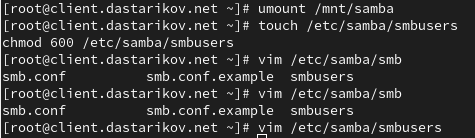
\includegraphics[width=0.8\textwidth]{../images/image22.png}
    \captionof{figure}{Отмонтирование каталога samba и создание файла smbusers.}
    \label{img:22}
\end{center}

\item На клиенте в файле /etc/fstab добавили следующую строку (Рис. \ref{img:23}):
    \begin{minted}{bash}
//server/sambashare /mnt/samba cifs user,rw,uid=dastarikov,gid=sambagroup, credentials=/etc/samba/smbusers,_netdev 0 0
    \end{minted}

\begin{center}
    \centering
    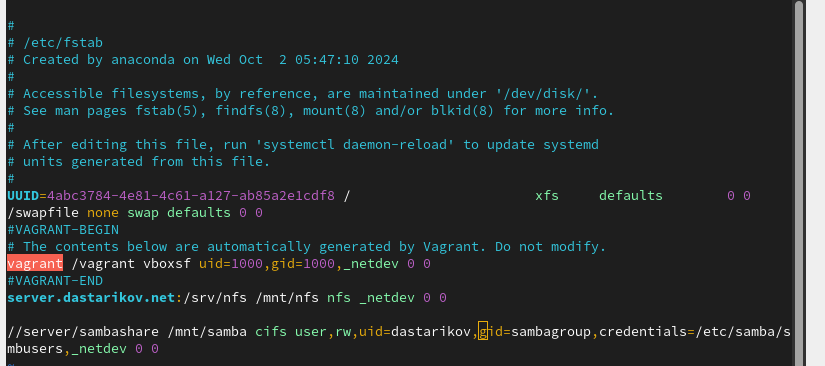
\includegraphics[width=0.8\textwidth]{../images/image23.png}
    \captionof{figure}{Изменение файла /etc/fstab.}
    \label{img:23}
\end{center}

\item Подмонтировали общий ресурс (Рис. \ref{img:24}):
    \begin{minted}{bash}
mount -a
    \end{minted}
\item Убедившись, что ресурс монтируется, перезагрузили клиента для проверки, что ресурс монтируется и после перезагрузки, а у пользователя есть доступ к разделяемым ресурсам (Рис. \ref{img:24}).

\begin{center}
    \centering
    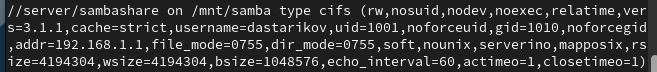
\includegraphics[width=0.8\textwidth]{../images/image24.png}
    \captionof{figure}{Настройка автоматического монтирования каталога для разделяемых ресурсов.}
    \label{img:24}
\end{center}

    \end{enumerate}
\end{enumerate}

\subsection{Внесение изменений в настройки внутреннего окружения виртуальных машин}
\begin{enumerate}
\item На виртуальной машине {\tt server} перешли в каталог для внесения изменений в настройки внутреннего окружения {\tt /vagrant/provision/server/}, создали в нём каталог {\tt smb}, в который поместили в соответствующие подкаталоги конфигурационные файлы (Рис. \ref{img:25}):
    \begin{minted}{bash}
cd /vagrant/provision/server
mkdir -p /vagrant/provision/server/smb/etc/samba
cp -R /etc/samba/smb.conf /vagrant/provision/server/smb/etc/samba/
    \end{minted}
\item В каталоге {\tt /vagrant/provision/server} создайте исполняемый файл {\tt smb.sh} (Рис. \ref{img:25}):
    \begin{minted}{bash}
cd /vagrant/provision/server
touch smb.sh
chmod +x smb.sh
    \end{minted}
Открыв его на редактирование, пропишите в нём следующий скрипт:
    \begin{minted}{bash}
#!/bin/bash
LOGIN=dastarikov
PASS=123456
echo "Provisioning script $0"
echo "Install needed packages"
dnf -y install samba samba-client cifs-utils
echo "Copy configuration files"
cp -R /vagrant/provision/server/smb/etc/* /etc
chown -R root:root /etc/samba/*
restorecon -vR /etc
echo "Configure firewall"
firewall-cmd --add-service samba --permanent
firewall-cmd --reload
echo "Users and groups"
groupadd -g 1010 sambagroup
usermod -aG sambagroup $LOGIN
echo -ne "$PASS\n$PASS\n" | smbpasswd -L -a -s $LOGIN
echo "Make share dir"
mkdir -p /srv/sambashare
chgrp sambagroup /srv/sambashare
chmod g=rwx /srv/sambashare
echo "Tuning SELinux"
semanage fcontext -a -t samba_share_t "/srv/sambashare(/.*)?"
setsebool samba_export_all_rw 1
setsebool samba_export_all_rw 1 -P
restorecon -vR /srv/sambashare
echo "Start smb service"
systemctl enable smb
systemctl start smb
systemctl restart firewalld
    \end{minted}

\begin{center}
    \centering
    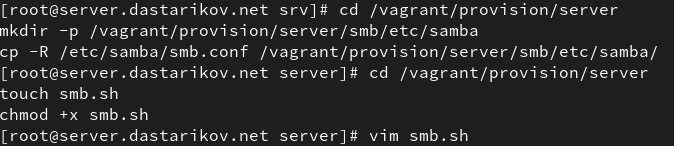
\includegraphics[width=0.8\textwidth]{../images/image25.png}
    \captionof{figure}{Изменение настроек внутреннего окружения на виртуальной машине server.}
    \label{img:25}
\end{center}

\item На виртуальной машине {\tt client} перешли в каталог для внесения изменений в настройки внутреннего окружения {\tt /vagrant/provision/client/}, создали в нём каталог {\tt smb}, в который поместили в соответствующие подкаталоги конфигурационные файлы (Рис. \ref{img:26}):
    \begin{minted}{bash}
cd /vagrant/provision/client
mkdir -p /vagrant/provision/client/smb/etc/samba
cp -R /etc/samba/smb.conf /vagrant/provision/client/smb/etc/samba/
cp -R /etc/samba/smbusers /vagrant/provision/client/smb/etc/samba/
    \end{minted}
\item В каталоге {\tt /vagrant/provision/client} создали исполняемый файл {\tt smb.sh} (Рис. \ref{img:26}):
    \begin{minted}{bash}
cd /vagrant/provision/client
touch smb.sh
chmod +x smb.sh
    \end{minted}
Открыв его на редактирование, прописали в нём следующий скрипт:
    \begin{minted}{bash}
#!/bin/bash
LOGIN=dastarikov
echo "Provisioning script $0"
mkdir -p /mnt/samba
echo "Install needed packages"
dnf -y install samba-client cifs-utils
echo "Copy configuration files"
cp -R /vagrant/provision/client/smb/etc/* /etc
chown -R root:root /etc/samba/*
restorecon -vR /etc
echo "Configure firewall"
firewall-cmd --add-service samba-client --permanent
firewall-cmd --reload
echo "Users and groups"
groupadd -g 1010 sambagroup
usermod -aG sambagroup $LOGIN
echo "Mounting dirs"
mkdir -p /srv/sambashare
echo "//server/sambashare /mnt/samba cifs user,rw,credentials=/etc/samba/smbusers,uid=user, gid=sambagroup,_netdev 0 0" >> /etc/fstab
restorecon -vR /etc
umount /mnt/samba
mount /mnt/samba
    \end{minted}

\begin{center}
    \centering
    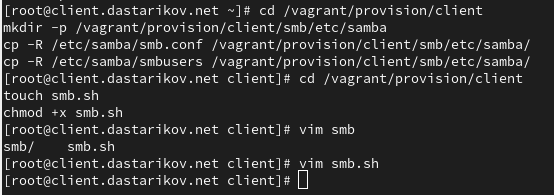
\includegraphics[width=0.8\textwidth]{../images/image26.png}
    \captionof{figure}{Изменение настроек внутреннего окружения на виртуальной машине client.}
    \label{img:26}
\end{center}

\item Для отработки созданных скриптов во время загрузки виртуальных машин {\tt server} и {\tt client} в конфигурационном файле {\tt Vagrantfile} добавили в соответствующих разделах конфигураций для сервера и клиента:
    \begin{minted}{bash}
server.vm.provision "SMB server",
type: "shell",
preserve_order: true,
path: "provision/server/smb.sh"
client.vm.provision "SMB client",
type: "shell",
preserve_order: true,
path: "provision/client/smb.sh"
    \end{minted}
\end{enumerate}

\section{Выводы}
В результате лабораторной работы познакомились с настройкой доступа групп пользователей к общим ресурсам по протоколу SMB.
\end{document}
